\subsection{Search Algorithms Used in CrowdHTN}
\label{improv: search algorithms}
As we have seen in our overview of different TOHTN planning techniques, the choice of algorithm and their behavior can have a big impact on performance. We see this in the varying behavior of planners relying on SAT-solving, DFS and heuristic search respectively. For this reason we wanted to explore the behavior of different search algorithms when applied to CrowdHTN.
As part of the re-engineering of CrowdHTN, we changed the implementation of the search algorithms to be based on a fringe. As mentioned in \cite{holler2020htn} we can simply switch out the underlying fringe data structure to emulate different search algorithms without making any changes to our core planner. Enabled by this change, we have implemented four search algorithms and will discuss them in the following section:
\begin{itemize}
	\item Random DFS
	\item Random BFS
	\item Heuristic DFS
	\item A*-like search
\end{itemize}
\begin{comment}
	- as mentioned in \cite{holler2020htn}, we can use a fringe-based implementation of progression search to swap out the fringe and realize different search strategies
	- the old implementation of Crowd did not properly do this, but we switched the implementation to allow us to test different algorithms here
\end{comment}

\subsubsection{Random Depth-First Search}
Random DFS is the only search algorithm that was already present in the previous implementation of CrowdHTN. It is implemented using a Last-In-First-Out queue as our fringe. Resolving an abstract task may create multiple new search nodes. If multiple nodes are created, we randomize their order before insertion into the fringe. This is done to avoid any pathological cases a fixed order may induce. We do not expect any differences in behavior or performance compared to the previous implementation.

\subsubsection{Random Breadth-First Search}
Random BFS is the first new search algorithm that we implemented. It is done by using a First-In-First-Out queue, allowing us to explore all the potential task hierarchies layer by layer. The insertion order of new nodes is randomized as in the DFS. We do this as the number of search nodes per layer can be exponential in the depth. As such, the last layer may dominate the overall work and the order in which we explore it can have a large impact on performance. \\
In general, we expect a higher memory footprint compared to DFS and assume that the planner will struggle with domains where plans are only found in deep layers or where the branching factor is very high as both will lead to a blowup in the size of our fringe and in the number of nodes we need to explore to find a plan. At the same time, we expect the performance of BFS to be more consistent than DFS, as the layer at which we find a plan stays fixed for any single instance. \\
Overall, we do not expect high performance of our BFS. It may however prove useful on some domains and help us understand and validate assumptions about the behavior of TOHTN problems.
\begin{comment}
- expect more memory
- worse performance
- will struggle with high branching factor or deep plans

- trivially complete, will always encounter everything
- reference statistics (branching factor from Crowd, minimal plan depth from Lilotane) to show that 

- probably not the best performance
- will help validate assumptions about TOHTN characteristics
\end{comment}

\subsubsection{Heuristic Search}
Both random DFS and BFS are unguided and do not adapt the order of search node exploration to information contained in those nodes. Other planners, such as PANDA, use heuristics to guide their search. We will describe search heuristics and their use in PANDA according to \cite{holler2020htn} and then go over how we try and adapt the use of heuristics with the added constraints of malleability.

\paragraph{Heuristics in hierarchical planning in general and PANDA specifically}
\label{improv: crowd heuristic}
The general idea of heuristic search is to explore our search space more intelligently. Heuristics achieve this by guiding the search to the most promising search nodes first.
In TOHTN planning, our choices during search are restricted by both the hierarchy of tasks as well as the world state. As a result, the best heuristics should make use of both pieces of information for the best results. \\
One avenue to deriving heuristics for HTN planning is to adapt classical planning heuristics. This proves difficult as these heuristics do not know about the hierarchy and may assume a state-based goal which HTN planning often does not have. To avoid these issues, PANDA instead adapts the hierarchical problem to match the heuristics. PANDA computes a classical planning problem which is a relaxation of the HTN problem at hand. Then a solution to this relaxed model is approximated with the help of classical planning heuristics and the result is used to guide the initial HTN planning procedure. The computation of the classical model is possible in polynomial time and only done fully in the beginning, afterwards the model is only updated for the current state of planning. As a result, the heuristic takes into account both hierarchy and world state with little overhead during search.
\begin{comment}
\cite{holler2020htn} (PANDA GBFS)
- heuristics allow us to not explore all of the search space
- hierarchy and world state both restrict our search, we should consider both, makes heuristic design difficult
- classical planning heuristics have problems:
- ignore the hierarchy
- heuristics have state-based goals, HTN not necessarily
- relax the HTN problem to classical planning (heuristic!) -> relaxed composition model
- uses actions and state of HTN problem
- adds reachability information
- then use another classical planning heuristic to solve the relaxed model
- use the resulting distance for HTN

- simplifications of the transformation:
- can use tasks that are not part of the decomposition hierarchy
- ordering constraints in decompositions are ignored
- each task task can only be introduced once and is then 'shared' in a way
- the size of the heuristic model is linear in the size of the input problem P
- computing the heuristic model is in $\mathcal{P}$
- update the model while searching

- heuristic is based on a grounded model
\end{comment}

\paragraph{Problems with the PANDA heuristic for malleable HTN planning}
While PANDA has managed to make great use of heuristics in HTN planning, we cannot simply adopt the same heuristics for malleable CrowdHTN. The reason for this lies in the assumption of PANDA that a ground problem instance is already available. Grounding is an expensive operation, though, as discussed in \cite{behnke2020succinct}. A full grounding may be exponential in size compared to the input and run times of grounding procedures are accordingly high. \\
While a grounding is already available in PANDA, CrowdHTN does not perform explicit grounding before planning. In a malleable environment without shared memory we can expect this grounding to take place every time a PE is added to a job, adding a high startup cost. A short-lived worker may be interrupted while still grounding, never starting the actual search. This would interfere with the efficient usage of available resources. For this reason we have decided against using the PANDA heuristics in CrowdHTN and instead tried to design a simpler heuristic to be used in malleable TOHTN planning.
\begin{comment}
- PANDA and its heuristics are great
- however, this imposes a startup cost
- implicitly assume a fully grounded instance (up to exponential size!)
- depending on instance grounding can take multiple minutes! (even for the efficient PANDA grounder up to 40 seconds)
- we perform this work multiple times, especially in a malleable environment
\end{comment}
\paragraph{A heuristic for malleable HTN planning}
To counter the startup cost of the PANDA heuristic, we have devised a simpler heuristic which is cheap to precompute and can easy to use in malleable planning. The goals are to have little startup overhead and to retain the efficient evaluation at each search step. As discussed in the previous paragraphs, this limits any precomputation to the lifted instance. We hope to still find performance gains on at least some problem instances. \\
As heuristic value, we use a lower bound on the number of reductions we still need to perform to fully resolve our list of open tasks. When computing this lower bound we ignore preconditions and effects, searching the shortest possible way through the hierarchy. We precompute this value for each task as described in algorithm \ref{algo: gbfs heuristic}. The heuristic value for each action is initialized to zero. The heuristic value for each abstract task is initially unknown. In each step we loop over all tasks $t$. For each method $m$ of task $t$ we check the heuristic value of all subtasks. The heuristic value of a method is set to the sum of the heuristic over all subtasks plus one. For each task we choose the minimum value over all corresponding methods. \\
Once there are no more changes in the mapping of tasks to heuristic values, we stop. Any task which at this point does not have an assigned value is not resolvable at all and can be pruned. \\
To visualize the computation of our heuristic, we provide an example TOHTN domain in figure \ref{figure: heuristic example} and table \ref{table: heuristic example} shows how the heuristic is computed on this domain. \\
Computing the final heuristic will take at most as many iterations as there are compound tasks. To show this we look at our hierarchical planning problem as graph. The tasks and methods form the vertices. We get edges from abstract tasks to all applicable methods and from methods to all their subtasks. Actions do not have any outgoing edges. During computation, the heuristic values are initialized at the actions and propagated and update throughout the graph. As tasks and methods alternate, any cycle contains at least one method and as such propagating the heuristic through a cycle would strictly increase it.\\
To evaluate our heuristic while planning, we now need to look at the whole sequence of open tasks and calculate the sum of our heuristic over those tasks. While the naive approach gives us linear run time in the number of open tasks, we can stretch the computation over task instantiation and reuse parts of it to perform heuristic evaluation in
\[
\mathcal{O}\left(\max \left\{ \# \text{subtasks of } m | m \in methods \right\} \right)
\] at run time. Details can be found in \ref{impl: efficient hashing} on efficient hashing of the open tasks, the technique also applies to the heuristic computation. Additionally, while we only use this heuristic to guide TOHTN planning, it ignores any orderings between open tasks. As such, it can be applied to HTN planning as well.
\begin{comment}
- inspired by PandaGBFS
- GBFS:
	- use a heuristic to grade each node
	- next node: best of all neighbors of the current node
	- then do a DFS on this
- GBFS is not complete
- might get stuck in an infinite loop
\todo{Quote to describe GBFS?}

The heuristic:
- use a heuristic that is cheap in both preprocessing and in computation during each step
- determine the minimum number of actions/ reductions needed to solve the task network
- ignore any and all parameters and world state to simplify the computation
\todo{ensure the code actually does this!}
- iterative approach:
	- initial:
		- actions have remaining depth 0
		- reductions without children/ where all children are noops have depth 1
	- iterating:
		- reductions: the sum of the minimum depths of all subtasks + 1
		- tasks: the minimum over all reductions
- i.e., we heuristically try to find nodes with the minimum amount of work remaining
- each iteration gives us the remaining depth of at least 1 compound task, else we terminate
- i.e., efficient to compute
- tasks that do not receive a value are unresolvable and can be pruned
\end{comment}
\begin{algorithm}
	\caption{GBFS heuristic calculation}
	\label{algo: gbfs heuristic}
	task depths $\gets \{(t_c, 0) | t_c \in \text{ concrete tasks}\}$\;
	\While{{\normalfont task depths} changed}{
		% get reduction depths
		\For{$t_c \in$ compound tasks}{
			reduction depths $= \emptyset$\;
			\For{$r \in$ reductions for $t_c$}{
				\If{depths of all subtasks are known}{
					reduction depths  = reduction depths $\cup 1 + \sum \{d | d \text{ is depth of a subtask of } r \}$\;
				}
			}
			
			\If{reduction depths $\neq \emptyset$}{
				task depths = task depths $\cup \{ (t_c, \min (\text{reduction depths})) \}$\;
			}
		}
	}
\end{algorithm}
\begin{figure}
	\caption{Example TOHTN domain to demonstrate our heuristic}
	\label{figure: heuristic example}
	\centering
	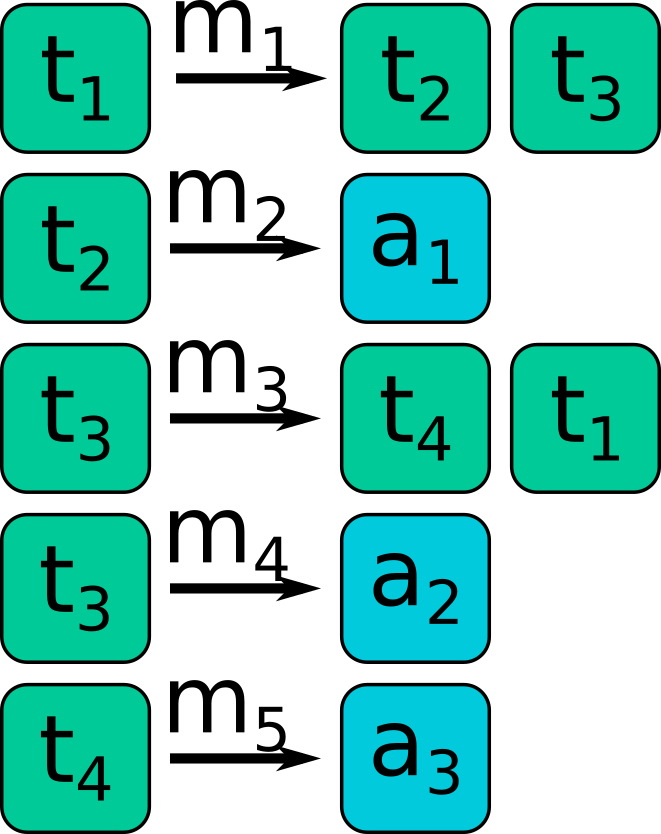
\includegraphics[width=0.3\textwidth]{images/final/heuristic_example}
\end{figure}

\begin{table}
	\caption{Example computation of our TOHTN heuristic for the domain in figure \ref{figure: heuristic example}. Changing values are bold.}
	\label{table: heuristic example}
	\centering
	\begin{tabular}{| c | c | c | c | c |}
		\hline
			  	& \multicolumn{4}{|c|}{Iteration} \\
		\hline
		task  	& 0			& 1 			& 2 			& 3 \\
		\hline
		$a_1$	& \textbf{0} 	& 0				& 0				& 0 \\
		$a_2$ 	& \textbf{0} 	& 0				& 0				& 0 \\
		$a_3$ 	& \textbf{0} 	& 0				& 0				& 0 \\
		$t_1$ 	&   			& 				& \textbf{3}	& 3 \\
		$t_2$ 	&   			& \textbf{1}	& 1				& 1 \\
		$t_3$ 	&   			& \textbf{1}	& 1				& 1 \\
		$t_4$ 	&   			& \textbf{1}	& 1				& 1 \\
		\hline
	\end{tabular}
\end{table}

\paragraph{Using the new heuristic in TOHTN planning}
With the new heuristic presented in the previous paragraph, we implemented two new search algorithms for CrowdHTN, those being a heuristic DFS and an A*-like search. \\
The implementation of DFS used so far performs the search in a uniformly random order. Without knowing anything about the domain, this is a reasonable choice. While it is far from optimal search, it also avoids any pathological cases that may arise from a fixed order of exploration. As an alternative to this random order, we used the heuristic to guide our DFS. We have to note that this is not necessarily fully deterministic. Randomness comes into play both when two reductions lead to search nodes with the same heuristic score - which happens e.g. for different instantiations of the same method - and when performing work stealing in a parallel setting. \\
In addition to the guided DFS, we also implemented an A*-like search where a node's value is the sum of the heuristic value and the number reductions applied to reach the node. We differ from A* in that we terminate the search as soon as a plan has been found instead of continuing on the search for an optimal plan. Our goal is for the heuristic to guide us towards a plan while giving weight to the number of applied reductions forces us to turn back and explore other parts of the search space without getting lost in endless loops due to pathological cases in our heuristic.

\subsubsection{Completeness of different Search Algorithms}
\label{improv: search completeness}
In the previous paragraphs we discussed a number of different search algorithms that we implemented for CrowdHTN and how we expect them to affect the performance characteristics of our planner. The search algorithm has a more fundamental impact than that, however, and may affect the completeness as well. In this section we want to give a short overview over the completeness of each of the algorithms. A summary is found in table \ref{table: search completeness}. Note that this discussion is only about the algorithms without any modifications. In section \ref{improv: loop detection} we discuss both loop detection and a restart mechanism and in section \ref{improv: completeness} we have a more detailed discussion about the completeness of different planners as well as the completeness of progression search with these additions. \\
DFS is not complete as it may enter an endless loop and, even if it still explores side-tracks from this loop, will never be able to backtrack out of the loop, cutting of parts of the search space. There is however always a chance to find a plan if it exists. I.e., there is a non-zero chance that the random choices all happen to be done correctly, the loop is never entered and a plan is found. \\
BFS on the other hand is trivially complete. While the exploration order within each layer is random we can provide an upper bound on the number of search steps required to explore a given search node $n$ on layer $i$. One such bound is the sum of all layer sizes from 0 up to and including $i$. \\
Next in our list is heuristic DFS. Similar to random DFS it may run into an endless loop. Compared to DFS, however, heuristic DFS may do so in a deterministic fashion if the domain triggers a pathological case in the heuristic. One example domain which would trigger such a case in our heuristic is visualized in figure \ref{figure: improv heuristic pathological}.
In this instance our heuristic assigns the value 1 to $m_1$, 2 to $m_2$ and 3 to $m_3$. If the preconditions of $m_1$ are not fulfilled, heuristic DFS will first try to resolve $t_1$ via $m_1$, fail, then use $m_2$ with the goal to try $m_1$ again afterwards. This will fail again and the loop is repeated indefinitely. While $m_3, m_4, m_5$ may provide a path out, they will never be used. \\ 
Lastly, we implemented A*-like search. While it does reuse the same heuristic, this algorithm achieves completeness by also valuing the number of applied methods so far. Let $n$ be a node with heuristic value $h$ and $r$ previously applied reductions to reach $n$. Then $n$ is guaranteed to be explored once all nodes with at most $h + r$ previously applied reductions have been explored. \\
All of this discussion so far has assumed sequential planners. The implications do hold for parallel search, too. For a planner using at most $n$ PEs we may always provide an instance with $n$ ways to enter an infinite recursion.
\begin{table}
	\caption{Completeness of the different search algorithms in CrowdHTN}
	\label{table: search completeness}
	\centering
	\begin{tabular}{| l | l |}
		\hline
		Algorithm & Completeness \\
		\hline
		Random DFS & Not complete. Positive probability to find a plan if it exists \\
		Random BFS & Complete \\
		Heuristic DFS & Incomplete \\
		A*-like & Complete \\
		\hline
	\end{tabular}
\end{table}
\begin{figure}
	\caption{A pathological case in our new HTN heuristic}
	\label{figure: improv heuristic pathological}
	\centering
	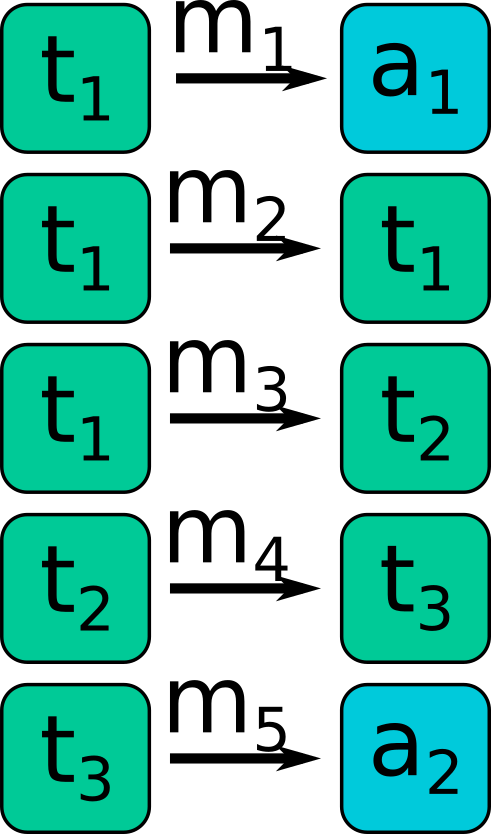
\includegraphics[width=0.2\textwidth]{images/final/heuristic_pathological}
\end{figure}

\begin{comment}
- dfs: may find any solution but may also run into the wrong direction
- bfs: definitely complete, each node has an easy upper bound for when it is reached
- gbfs: may not find a plan at all if a heuristic is sufficiently pathological on an instance, leading into an endless loop
- astar: complete, distance travelled forces some bfs-like characteristics back into our exploration leading to completeness
\end{comment}
